\subsection{Descrizione generale}
Durante la fase di progettazione, il gruppo lineCode ha deciso di modellare l'architettura generale in quattro moduli distinti:
\begin{itemize}
	\item \textbf{server}: motore di calcolo che coordina le unità e genera le informazioni per la UI. Viene modellato seguendo la \textit{layered architecture};
	\item \textbf{interfaccia grafica}: mostra la mappa e permette di gestire le unità e gli utenti. Viene modellato seguendo la \textit{MVVM};
	\item \textbf{unità}: si occupa di simulare il comportamento di un'unità all'interno dell'ambiente. Viene modellato seguendo la \textit{hexagonal architecture};
	\item \textbf{sensori}: si occupa di simulare il comportamento dei sensori delle unità all'interno dell'ambiente. Non viene modellato secondo una architettura specifica poiché triviale.
\end{itemize}
La UI e l'unità comunicano con il server tramite l'uso di \glock{WebSocket} e lo scambio di messaggi \glock{JSON}. Il server quindi, conoscendo la posizione di tutte le unità e ostacoli, genera il percorso migliore e lo comunica alle unità richiedenti e aggiorna la mappa informando l'interfaccia grafica. 
Di seguito rappresentiamo l'architettura generale progettata. 

\begin{figure}[H]
	\centering
	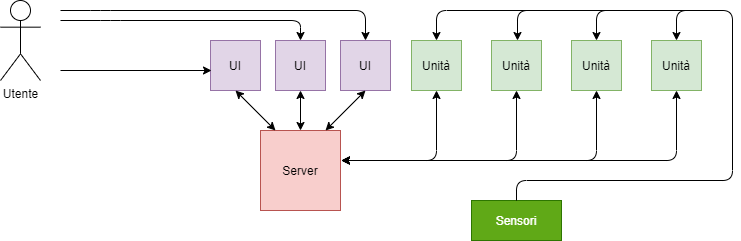
\includegraphics[width=16cm]{img/arch_generale.png}
	\caption{Architettura generale}
\end{figure}
